\chapter{The OpenRobots Ontology Framework}
\label{chapt|oroserver}

This chapter introduces the \emph{OpenRobots Ontology} server and its
common-sense knowledge base.

We present here the functional description of {\tt oro-server}, and detail
its knowledge model. Its actual implementation is discussed in the next
chapter.

We also present the \emph{OpenRobots Common-Sense Ontology} that contains most
of the knowledge at hand when the robot starts.

\section{Functional overview}
\label{sect|functional-overview}

We have adopted a centralised approach for knowledge management called
ORO~\cite{Lemaignan2010}. The platform is designed as a central
knowledge storage service implemented as a server where the robot
components can add or query statements at run-time. Figure~\ref{fig|oro-overview}
illustrates the main functional components of ORO.

\begin{figure}
\centering
  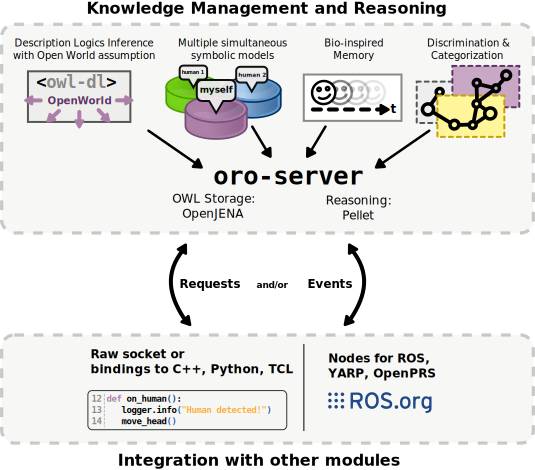
\includegraphics[width=0.75\columnwidth]{oroserver/oro_architecture_functional.pdf}
  \caption{Overview of the ORO architecture.}
  \label{fig|oro-overview}
\end{figure}

At the core, ORO is build around the
OpenJena\footnote{\url{http://www.openjena.org}} ontology management library,
connected to the Pellet\footnote{\url{http://clarkparsia.com/pellet}}
reasoner.

A front-end accepts and manages connections to clients. The clients' requests
are processed by a set of internal modules: basic operations on statements, but
also higher cognitive and human-robot interaction related features are
available. External plugins can also be added via a specific extension
mechanism.

Besides acting as a facts database, the ORO platform exposes several
functions: operations on knowledge statements relying on inference (through a
continuous first-order logic classification process), management of
\emph{per-agent} symbolic models, categorisation of sets of concepts
and profiles of memory (that enable the robot to ``forget'' about some facts).

ORO also provides an event mechanism that allows components to be triggered
when specific events occur. A component can for instance subscribe to events
of kind \setstmt{?agent isVisible true, ?agent type Human}. As soon as the
perception layer detects a human in the robot's field of view and accordingly
updates the knowledge base, the executive layer is triggered. The event
framework also takes advantage of the inference capabilities of ORO. Thus an
event can be indirectly triggered if its triggering conditions can be
inferred to be true.



%%%%%%%%%%%%%%%%%%%%%%%%%%%%%%%%%%%%%%%%%%%%%%%%%%%%%%%%%%%%%%%%%%%%%%%%%%%%%%%
%%%%%%%%%%%%%%%%%%%%%%%%%%%%%%%%%%%%%%%%%%%%%%%%%%%%%%%%%%%%%%%%%%%%%%%%%%%%%%%

\section{The ORO knowledge model}
\label{sect|knowledge-model}

\subsection{Expressiveness}
\label{sect|oro-expressiveness}

Unlike systems relying on logic programming, ORO is purely
based on Description Logics: the ORO knowledge model is based on RDF triples
(\ie exclusively binary predicates). Triples \stmt{subject predicate object}
are the atoms of knowledge for ORO.

Knowledge in the ORO server is represented with OWL2. As already mentioned at
section~\ref{sect|std-reasoning}, the available constructs include:

\begin{itemize}
    \item inheritance relations, \eg: \par
    \stmt{Bottle subClassOf Container} $\models$ \emph{all bottles are containers},

    \item property axioms
        \begin{itemize}

        \item specification of predicates' domain and range, \eg:\par
        \stmt{thinksAbout domain IntelligentAgent} $\models$ \emph{only
        intelligent agents can think},

        \item cardinality constraints (including \concept{allValue}, 
        \concept{someValue}, \concept{hasValue}),

        \item property characteristics (symmetry, transitivity, reflexivity,
        antisymmetry, etc.)

        \end{itemize}

    \item class restrictions like: \par \concept{Bottle} $\equiv$
        \concept{Artifact} {\bf that} (\concept{hasShape} {\bf value}
        \concept{cylinderShape})

    \item set operations like: \par \concept{Color} $\equiv$ {\bf unionOf}(\concept{blue},
        \concept{green}, \concept{orange}, \concept{black}...)
\end{itemize}

DL-safe\footnote{In DL-safe rules, variables bind only to explicitly named
individuals in the ontology.} SWRL ({\em Semantic Web Rule Language}) rules are
also supported. For example: \par
        \concept{looksAt(?agt, ?obj)} $\land$
        \concept{pointsAt(?agt,?obj)} $\Rightarrow$ \concept{focusesOn(?agt, ?obj)}


The formal expressiveness of the current version of the ORO common-sense
ontology (commit {\tt 19f1fcf27} in the public repository\footnote{Clonable
from \url{http://git.openrobots.org/git/robots/oro.git}}) is
$\mathcal{SROIQ(D)}$, which correspond to the OWL2 language full expressiveness (the
appendix~\ref{chapt|dl} presents the usual naming conventions of Description
Logics expressiveness).

Table~\ref{table|onto-stats}, page~\pageref{table|onto-stats} gives
quantitative details on the type of axioms used in the ORO common-sense
ontology.

\paragraph{Reification} Since RDF triples constrain to binary predicates,
\emph{reification} is often required to express $n$-ary relations. For
instance, the relation \emph{A gives object B to C} can not directly be
represented in RDF. This relation is reified as \{\stmt{act1 type Action},
\stmt{act1 performedBy A}, \stmt{act1 actsOn B}, \stmt{act1 receivedBy C}\}. As
long as the instance \concept{act1} exists in the knowledge base, the original
relation \emph{A gives object B to C} is considered to hold. This kind of
reification is common in the ORO knowledge model.

Reification can also take place at a meta-level (this is the level usually
intended by the term reification): a triple \stmt{subject predicate object} can
be itself reified in \{\stmt{stmt1 type Statement}, \stmt{stmt1 hasSubject
subject}, \stmt{stmt1 hasPredicate predicate}, \stmt{stmt1 hasObject object}\}.
This level of reification allows to characterise the knowledge atoms
themselves, for instance to specify when the atom was added. The section on
memory management in ORO server, below, gives examples of usage of this
meta-cognition feature.

Note that in traditional logical programming like Prolog, reification is rarely
strictly required since no constraints hold on the arity of predicates. To
store the date of creation of a facts, one could simply add it as a
supplementary argument of the predicate\footnote{In the case of time
representation, however, reification --- or, in the case of logic programming,
second order logic --- often takes place through the \emph{fluents} mechanisms,
see section~\ref{sect|time-representation}}.

\paragraph{Open World Assumption}

Following the OWL language model and as mentioned at
section~\ref{sect|owa-cwa}, the ORO knowledge model makes the open world
assumption.

This allows to easily represent that a fact is unknown (by simply not stating
it in the knowledge base), but also requires to carefully explicit what the
entities are and are not.

%%%%%%%%%%
\subsection{Special representation techniques}

\subsubsection{Representation of alternative knowledge models}
\label{sect|alterite}

As pictured in Figure~\ref{fig|oro-overview}, ORO stores independent cognitive
models for each agent it interacts with. When the ORO server actually
identifies a new agent (or infers that some instance is an agent), it
automatically creates a new, separate, in-memory OWL model for that agent.
Then, different robot components, like execution control or situation
assessment, may store the agents' beliefs in separate, independent models. All
knowledge processing functions in the robot's primary model are equally
available in every agent's model, which allows us to store and reason on
different (and possibly globally inconsistent) models of the world.

Each of these models is independent and logically consistent, enabling
reasoning on different perspectives of the world that would otherwise be
considered as globally inconsistent (for instance, an object can be visible for
the robot but not for the human. This object can have at the same time the
property \concept{isVisible \textit{true}} and \concept{isVisible
\textit{false}} in two different models).

We present at section~\ref{sect|spark}, page~\pageref{sect|spark}, a 3D
real-time environment, SPARK, that allows to compute on-line several symbolic
properties that are dependent on the perspectives.

\paragraph{Theory Of Mind and contexts} \label{sect|theory-of-mind}

By maintaining independent mental states for each agent it interacts with, we
consider the robot to be endowed with a simple \emph{theory of
mind}~\cite{Scassellati2002}: the robot can explicitly model the beliefs of its
interactors, it expose them to the control architecture, and the same set of
cognitive abilities are available on these secondary model as on the main
model: reasoning, inconsistencies detection, events, etc.

Proper \emph{false beliefs} experiment, similar to the Sally and Ann experiment
presented in the previous chapter, has been recently conducted with ORO
by Mathieu Warnier, as reported in~\cite{Warnier2012a}: in this experiment, two
humans observe a table with several objects, then one leaves while the other
one moves around some objects. This leads to two different set of beliefs on
the world, which the robot explicitly stores and updates when necessary (if the
human comes back and check the table, for instance).

These multiple models can also be viewed as different \emph{interpretive
frames}, allowing the robot to interpret the same reality from different points
of view. In this sense, each model carries a context of interaction.  In
chapter~\ref{chapt|dialogs}, we present how such agent-dependent contexts are
used by a natural language processor to make sense of user sentences from
his/her point of view.

\subsubsection{Multi-lingual support}
\label{sect|multilingual}

The RDF specification supports internationalisation by the way of
\emph{language tags}: plain literals may have an optional language tag (taken
from the standard RFC-3066) that tells in which human language the literal is
expressed.

ORO benefits from this mechanism, and can be configured to use a specific
language as default. When an language is explicitly selected, the translated
labels of concepts (when available in the underlying ontology) are used instead
of the default English ones.

Since only the labels (\ie the human-friendly name of the concepts) are subject
to translation, changing the default language of the ORO server has no semantic
impact: entities in the ontology always refer to same concepts. Same inferences
are drawn, same connections to knowledge sources are made, etc. The strength of
semantic approaches is here well illustrated.

%%%%%%%%%%
\subsection{Reasoning techniques}

\subsubsection{Standard inference services}

As explained in the next chapter, we use the Pellet open-source reasoner to
reason on the knowledge base. This enables to expose several standard inference
services: consistency checking, concept satisfiability, classification and
realisation (the most specific classes that an individual belongs to).

In case of inconsistency in one of the knowledge models stored by ORO, an explanation
of the inconsistency is proposed, in a human-readable form, for debugging
purposes. The automatic exploitation of the explanation by the robot executive
controller is yet to be developed.

\subsubsection{Grounding, classification and discrimination algorithms}
\label{sect|discrimination}

ORO server implements several algorithms to identify similarities and
differences between concepts (classes or instances)~\cite{Ros2010b}. The main
ones are presented in this section.

\paragraph{Common and first different ancestors} The \emph{Common Ancestors}
algorithm (algorithm~\ref{algo|common-ancestors}) returns the classes that
are the ``first'' common super-classes of the two concepts.

\begin{figure}
    \centering
    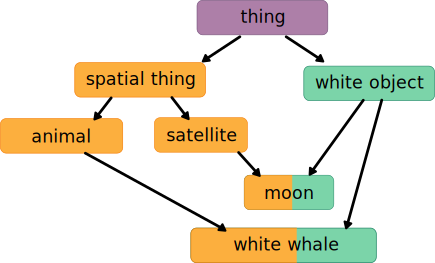
\includegraphics[width=0.6\columnwidth]{oroserver/commonancestors.pdf}
    \caption{Sample taxonomy to illustrate \emph{common ancestors} algorithms.}
    \label{fig|common-ancestors}
\end{figure}

\small
\begin{pseudocode}[ruled]{CommonAncestors}{concept1, concept2}
\label{algo|common-ancestors}

\BEGIN
\mathcal{I} \GETS \CALL{Superclasses}{concept1} \cap \CALL{Superclasses}{concept2} \\
\RETURN {c \in \mathcal{I} | \CALL{Subclasses}{c} \cap \mathcal{I} = \emptyset}\\
\END

\end{pseudocode}
\normalsize

Taking the taxonomy in figure~\ref{fig|common-ancestors} as example, the common
ancestors for the pair \concept{\{white whale, moon\}} are
\concept{\{spatial thing, white object\}}, \ie the set of classes that belong to
the intersection of the super-classes of both the concepts and that have no
sub-classes in this intersection.

The common ancestors are useful  to determine the most precise class(es) that
include a given set of individuals.

\small
\begin{pseudocode}[ruled]{FirstDifferentAncestors}{concept1, concept2}
\label{algo|first-different-ancestors}

\BEGIN
\mathcal{C} \GETS \CALL{CommonAncestors}{concept1, concept2} \\
\mathcal{S} \GETS \CALL{Superclasses}{concept1} \cup \CALL{Superclasses}{concept2} \\

\RETURN{\forall c \in \mathcal{C}, \CALL{DirectSubclasses}{c} \cap \mathcal{S}} \\
\END

\end{pseudocode}
\normalsize

The \emph{First Different Ancestors} algorithm
(algorithm~\ref{algo|first-different-ancestors}) returns the list of direct
sub-classes of the common ancestors. They are intuitively the most generic
types that \emph{differentiate} the two concepts. In the taxonomy
figure~\ref{fig|common-ancestors}, two instances \concept{a} and \concept{b} of
respectively \concept{white whale} and \concept{moon} have as first different
ancestors the two sets \concept{\{animal, satellite\}} (subclasses of ancestor
\concept{spatial thing}) and \concept{\{white whale, moon\}} (subclasses of
ancestor \concept{white object}).

\paragraph{Clarification Algorithm}
\label{sect|clarify}

During interactions with other agents, the robot is often required to figure
out which individual correspond to a description like ``red object'', ''a
bottle'', ''a book larger than this other one'', etc. This is a key part of the
grounding capability.

Clarification and discrimination algorithms are based on what we call
\emph{descriptors}: descriptors can be properties of individuals, either
acquired by the robot are statically asserted in a common-sense ontology. They
are also the result of other reasoning algorithms like the \emph{Common
Ancestors} and \emph{Different Ancestors} algorithms presented above.
We shall see later how symbolic knowledge is first acquired from geometric
reasoning or natural language processing, and we consider in this section that
the \emph{clarification} process is based on an established ontology, like the
sample proposed in figure~\ref{fig|discriminant}.

Based on this ontology and a given partial (or complete) description of an
object (list of attribute-value pairs), the robot is able to identify the
referred object the following way (Algorithm~\ref{algo|clarify}). First it
obtains all objects that fulfil the initial description by querying the agent
model in the knowledge base. Based on the result it either succeeds (obtains
one single object), fails (no object with that description could be found) or
obtains several objects. In this last case, a new descriptor is added
(mark~\ref{clar.desc}) to the initial description and the process starts over
again until all possible descriptors have been added.

Failure occurs hence in two cases: when the description does not match any object
from the robot's knowledge, either because the robot's knowledge is incomplete
(the human refers to an unknown descriptor or descriptor value), or when a set of
candidates could not get successfully discriminated with the available
descriptors.

Two options are available to add new descriptors: directly asking the human for
more information, or automatically searching a new attribute and ask the human
for its value. In the latter case, we need to automatically find the best
discriminant for the current list of objects being evaluated ($candidates$ in
the algorithm).


\small
\begin{pseudocode}[ruled]{Discrimination}{description, agent}
\label{algo|clarify}
\BEGIN
candidates \GETS \CALL{GetObjectFromDescription}{description, agent} \\
\IF \left|{candidates}\right| = 1 \THEN \RETURN{candidates[0]} \\
\ELSEIF \left|{candidates}\right| = 0 \THEN \OUTPUT{\mbox{No object found!}} \\
\ELSE
    \BEGIN
        description \GETS \CALL{AddDescriptor}{description, agent} \STMTNUM{7em}{clar.desc}\\
        \RETURN{\CALL{Discrimination}{description, agent}} \\
    \END
\END

\end{pseudocode}
\normalsize

\paragraph{Finding a discriminant}
\label{sect|discriminant}

\begin{figure}
    \centering
    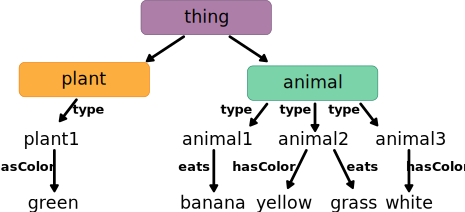
\includegraphics[width=0.7\columnwidth]{oroserver/discriminant.pdf}
    \caption{Sample ontology to illustrate the discrimination routines.
    \concept{plant1} is an instance of \concept{Plant} and
    \concept{animal[1-3]} are instances of \concept{Animal}.}
    \label{fig|discriminant}
\end{figure}

We have implemented a set of semantic categorisation functions in ORO. One of
them consists in looking for discriminants, \ie descriptors that allow a
maximum discrimination among a set of individuals.

We distinguish two types of discriminants. \emph{Complete} discriminants are
those attributes (or properties) that totally discriminate the set of
individuals. In other words, properties whose values can uniquely identify
those individuals. However, they are not always available. First, because two
or more individuals may share the same value, and second, because not all
individuals may share the same properties. Thus, \emph{partial} discriminants
are those that split at best the set of individuals in different subsets
based on some criteria.

\small
\begin{pseudocode}[ruled]{GetDiscriminant}{individuals}
\label{algo|discriminant}
\BEGIN
P \GETS \CALL{Ontology.GetProperties}{individuals} \\
\hat{P} \GETS \emptyset \\
\FOREACH p \in P \DO
    \BEGIN
        n_{ind} \GETS \CALL{NbIndividualsWithProperty}{p} \STMTNUM{7em}{disc.nbind}\\
        n_{val} \GETS \CALL{NbDifferentValues}{p} \STMTNUM{10.9em}{disc.nbval}\\
        \IF n_{val} > 1 \THEN
            \hat{P} \GETS \CALL{Append}{[p,n_{ind},n_{val}]} \STMTNUM{8.8em}{disc.append}\\
    \END \\

\CALL{Rank}{\hat{P}} \STMTNUM{23.6em}{disc.rank}\\
\RETURN{\hat{P}[0][0]} \\
\END

\end{pseudocode}
\normalsize

The algorithm to determine the type of discriminant available
(Algorithm~\ref{algo|discriminant}) has the following steps (to better follow
it, we base its description on the ontology example illustrated in
figure~\ref{fig|discriminant}). We search a discriminant for the following
individuals: \concept{plant1}, \concept{animal1}, \concept{animal2} and
\concept{animal3}. First we obtain the direct properties and classes for all
the individuals, \ie we do not consider all the hierarchy of properties and
classes (in the example, \concept{plant1} has two super-classes
(\concept{Plant} and \concept{Thing}), but we only take the most direct one
(the class \concept{Plant})). Next, we compute the number of individuals per
property (mark~\ref{disc.nbind}) and the number of different values for that
property (mark~\ref{disc.nbval}). For instance, for the property
\concept{type}: all the four instances have a type, $n_{ind} = 4$, and this
property has two possible values (\concept{Plant} and \concept{Animal}),
$n_{val} = 2$. If $n_{val} > 1$ (in other words, if not all individuals have
the same value), then we consider that property as a potential discriminant
(mark~\ref{disc.append}).  Finally, we rank (mark~\ref{disc.rank}) the list of
potential properties following two criteria: the number of individual
occurrences (\ie we maximise the coverage of that property) and the values
occurrences (\ie the more distinct values, the better).  The best discriminant
corresponds to the first element of the sorted list. In other words, the class
with higher number of occurrences and more variety in it.  If several
properties are equal, we return all of them.

In our example, the algorithm would return the type as best the partial
discriminant. If we only consider the instances of the class \concept{Animal},
it would return two properties equally discriminant: \concept{hasColor} and
\concept{eats}.

We use this algorithm in particular for interactive concept grounding. We will
detail this approach at chapter~\ref{chapt|dialogs}.

\subsubsection{Memory}
\label{sect|oroserver-memory}

The ORO server offers a mechanism to mimic simple forms of biological memory.
When new statements are inserted in the knowledge base, a \emph{memory profile}
is optionally attached to them.

Three such profiles are predefined: {\tt short term}, {\tt episodic} and {\tt
long term}. They each correspond to a different lifetime for the statements
(respectively 10 seconds, 5 minutes and no time limit). After this duration,
the statements are automatically removed from the knowledge base.

This approach is limited. In particular, \emph{episodic} memory primarily refers
to the semantics of the statements (that is expected to be related to an event)
and not to a specific life duration. We discuss at the end of this work possible
improvements.

\paragraph{Active Concepts} We rely however on this short term memory for a
particular use-case:  \emph{active concept}. Some modules, like our natural
language processor (described at chapter~\ref{chapt|dialogs}), use
the {\tt short term} memory profile to mark for a few seconds important
concepts that are currently manipulated by the robot. For example, if a human
asks the robot: ``Give me all red objects'', the human, the \concept{Give}
action, and each red objects that are found are successively marked as
\emph{active concepts} by inserting statements like \stmt{human type
ActiveConcept} in the short-term memory (which can be considered, in this case,
to be a working memory, as defined at section~\ref{sect|memory}). We use this
feature to give a (visual) feedback to the users (section~\ref{sect|oroview})

\subsubsection{Knowledge structure alteration and learning}

In the ORO server, the knowledge structure (\emph{TBox}) is purely declarative
and asserted as regular statements (like \stmt{Location subClassOf
SpatialThing}), following the RDF Schema (RDFS) and OWL language constructs.

In complement to the constructs already presented at
section~\ref{sect|oro-expressiveness}, table~\ref{table|main-tbox-properties}
lists the main properties and classes defined in RDFS and OWL that allow to
describe the ontology structure. These constructs can all be inserted at
run-time to alter the knowledge model of the server. They are immediately taken
into account by all reasoning process taking place after this point.

\begin{table}
\begin{center}

\begin{tabular}{ll}
\toprule
{\bf Name} & {\bf Example} \\
\midrule
{\tt rdfs:subClassOf} & \stmt{Human subClassOf Agent} \\
{\tt rdfs:subPropertyOf} & \stmt{hasColor subPropertyOf hasFeature} \\
{\tt rdfs:domain} & \stmt{thinks domain IntelligentAgent} \\
{\tt rdfs:range} & \stmt{name range string} \\
{\tt owl:inverseOf} & \stmt{sees inverseOf seenBy} \\
{\tt owl:FunctionalProperty} & \stmt{age type FunctionalProperty} \\
{\tt owl:TransitiveProperty} & \stmt{isAbove type TransitiveProperty} \\

\bottomrule

\end{tabular}
\end{center}

\caption{Some of the properties and classes defined in RDFS and OWL that allow
to define the semantics and relations of terms within an ontology.}

\label{table|main-tbox-properties}
\end{table}


While we do not claim to have addressed the issue of learning in general, TBox
alteration coupled with language processing features, enables to implement
specific learning mechanisms.  For example, one can teach the robot that cats
are animals by processing a sentence like ``Cats are animals'' into \stmt{Cat
subClassOf Animal} and then adding it at run-time into the knowledge base. From
that points, all entities asserted or inferred to be cats will be as well
inferred to be animals.

The case study \emph{Point \& Learn} (section~\ref{expe|pointandlearn})
presents some experimental results in this domain.

\subsubsection{Fast concept lookup}
\label{sect|oroserver-lookup}

Because retrieving a concept from its label (for instance, a ``location'' is
the human label for the concept \concept{cyc:SpatialThing-Localized}) is a
frequent operation, in particular for language processing application, the ORO
server also provides a fast concept look-up mechanism to search for a concept
identifier by its label. This also takes into account the chosen language
(English, German, French...).

%%%%%%%%%%%%%%%%%%%%%%%%%%%%%%%%%%%%%%%%%%%%%%%%%%%%%%%%%%%%%%%%%%%%%%%%%%%%%%
%%%%%%%%%%%%%%%%%%%%%%%%%%%%%%%%%%%%%%%%%%%%%%%%%%%%%%%%%%%%%%%%%%%%%%%%%%%%%%
%%%%%%%%%%%%%%%%%%%%%%%%%%%%%%%%%%%%%%%%%%%%%%%%%%%%%%%%%%%%%%%%%%%%%%%%%%%%%%

\section{Knowledge instantiation: the OpenRobots Common-Sense Ontology}
\label{sect|oro-commonsense}

The ORO platform is made of the server that we have presented, and a
common-sense ontology, the \emph{ORO Common-sense Ontology}.

At start-up, the knowledge model of the ORO server is initialised with a
configurable sets of ontologies that build together the initial pool of facts
known to the robot: the common-sense ontology and optional, domain dependent
ontologies.

Each time a new model is created (typically when a new agent is detected), it
is also initialised with the same pool of facts.  From the point of view of the
robot, this ensure that all the different agents share the same background
knowledge.

Usually, the ORO server is started with the common-sense ontology that we
present in this section, and one scenario-specific ontology that usually
contains the set of individuals with relevant properties needed by the
experiment.

\begin{table}
\begin{center}

\begin{tabular}{ll}
\toprule
Expressiveness & $\mathcal{SROIQ(D)}$ \\
Axioms & 961 (annotations: 359)\\
Class count & 108 \\
Object property count & 78 \\
Data property count & 13 \\
Individual count & 21 \\
Functional properties & 19 \\
Inverse properties & 9 \\
Transitive properties & 4 \\
Symmetric properties & 3 \\
\bottomrule

\end{tabular}
\end{center}

\caption{Statistics on the ORO common-sense ontology.}

\label{table|onto-stats}
\end{table}

The table~\ref{table|onto-stats} gives a first overview of the extend and
expressive level of the ORO common-sense ontology. While the raw numbers of
axioms is in no way comparable to large upper ontologies (as presented at
chapter~\ref{chapt|krs}), the modeling is also more expressive (with the use of
second order predicates) than the ontologies that are partially or completely
generated automatically.

\begin{figure}
    \centering
    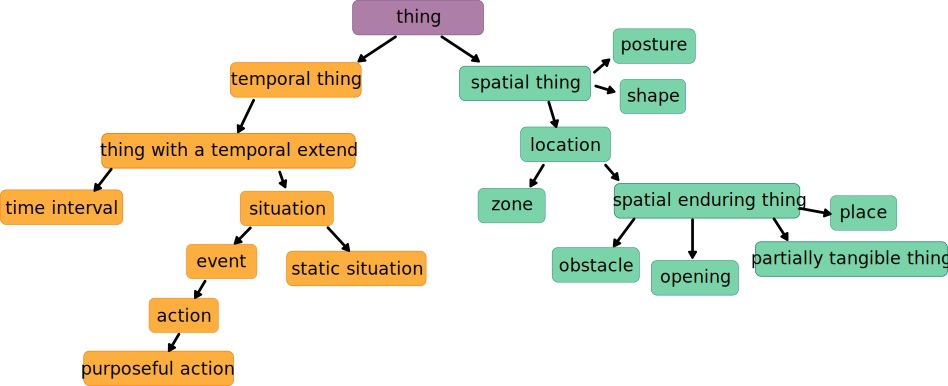
\includegraphics[scale=0.6]{oro/top_tbox.pdf}

    \caption{The upper part of the ORO common-sense TBox. All these concepts
    belong to the {\sc OpenCyc} namespace.}
    
    \label{fig|upper_tbox}
\end{figure}

The ORO common-sense ontology has been designed from two requirements: covering
our experimental needs and conforming as much as possible to the {\sc OpenCyc}
upper ontology.

This lead to a bidirectional design process: from \emph{bottom-up} regarding
the choices of concepts to model, \emph{top-down} regarding the upper part of the
taxonomy. This upper part of the ontology is pictured on
figure~\ref{fig|upper_tbox}. All the classes visible on this figure belong to the
{\sc OpenCyc} namespace (the {\tt cyc:} prefix is omitted).

By \emph{aligning} the upper part of the ontology on {\sc OpenCyc} (as other
KRS, like {\sc KnowRob} or PEIS K\&R, did) has multiple advantages. First the
design of this part of the ontology is generally difficult: it pertains to
abstract concepts whose mutual relations comes to philosophical debates. The
upper taxonomy of {\sc OpenCyc} represents a relative consensus, at least
within the semantic Web community. Then, because it is a well established
project with numerous links to other on-line databases (like Wikipedia or
WordNet), the reuse of important {\sc OpenCyc} concepts ensures to a certain
extend that the knowledge stored by the robot can be shared or extended with
well-defined semantics. A good example is the concept of \emph{Object}: In
everyday conversation, an object is a relatively small physical thing, that can
be typically manipulated. Normally, a human is not considered as an object. In
{\sc Cyc}, an object has a more precise definition: it is something
\emph{partially tangible}. That includes obviously the humans, and actually
many other entities that would not be commonly said to be objects (the Earth
for instance). Thus the importance of relying on well-defined and standard
semantics to exchange informations between artificial systems.

This figure~\ref{fig|upper_tbox} also illustrates the fundamental disjunction
in the ORO model between \emph{temporal} and \emph{spatial} entities (formally,
$(TemporalThing \sqcap SpatialThing)^{\mathcal{I}} = \emptyset$, with
$\mathcal{I}$ the \emph{interpretation} of our model).

The class \concept{purposeful action} is the superset of all the actions that
are voluntarily performed by the robot (or another agent). Subclasses (like
\concept{Give}, \concept{LookAt}, etc.) are not asserted in the common-sense
ontology, but are added by the execution controller (in link with the symbolic
task planner) and the natural language processor based on what is actually
performable and/or understandable by the robot at run-time.

The tree of figure~\ref{fig|upper_tbox} (this subset of the ontology is indeed
a tree: this has however not to be the case in general, and, as a matter of
fact, the TBox of the whole ORO common-sense ontology does not form a tree) is
not equally developed at lower levels. We have already briefly mentioned the
developments of the actions. The other important part is the descendants of the
\concept{partially tangible thing} (what is commonly called an \emph{object}).
Figure~\ref{fig|tangible_things_tbox} gives more details on this part of the
ontology.

\begin{figure}
    \centering
    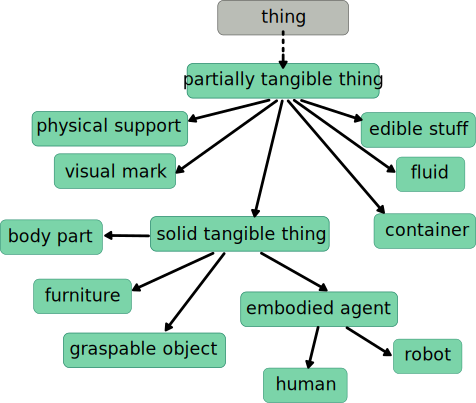
\includegraphics[scale=0.6]{oro/tangible_things_tbox.pdf}
    \caption{TBox of the specialisations of \concept{PartiallyTangible}.}
    \label{fig|tangible_things_tbox}
\end{figure}

This excerpt from the ontology makes the bottom-up design process visible: only
few types of \emph{partially tangible} things appear, and only subclasses
relevant to the context of service robotics in an human-like environment are
present.

Lastly, the ORO common-sense ontology contains several rules and class
expressions that encode non-trivial inferences.

The definition of the \concept{Bottle} is a case in point. We already gave a
simplified version, here the complete definition:

\concept{Bottle} $\equiv$ \concept{Container} {\bf and} \concept{Tableware}
{\bf that} (\concept{hasShape} {\bf value} \concept{cylinderShape} {\bf and}
\concept{hasCharacteristicDimension} {\bf only} \concept{\em int[>= 0.1, <=
0.3]})

If a human informs the robot that a given object is indeed a bottle, the robot
can then infer much more on this object. And if the human affirms that a car is
a bottle, the robot may question this assertion because of the inconsistent
size.

%%%%%%%%%%%%%%%%%%%%%%%%%%%%%%%%%%%%%%%%%%%%%%%%%%%%%%%%%%%%%%%%%%%%%%%%
%%%%%%%%%%%%%%%%%%%%%%%%%%%%%%%%%%%%%%%%%%%%%%%%%%%%%%%%%%%%%%%%%%%%%%%%
\recap

We conclude here this third chapter. This chapter was focused on the functional
and algorithmic presentation of the ORO server, a \emph{semantic blackboard}
where robotic modules can write and querying pieces of knowledge.

We have mentioned how multiple mental models can be managed by the server, and
we have also presented several active services, like the discrimination
algorithms or the management of the memory.

Finally, we have presented the ORO \emph{common-sense} ontology that provide
the robot with an initial background knowledge, shared by all the agents.

The next chapter first gives some implementation and technical details about
the ORO framework, and then present how ORO is integrated with other components
on real robots. In particular, we detail the integration with the geometric
reasoning module and the symbolic task planner.


